\section{Use Cases and Scenarios}
\label{sec:use-cases}

Fig.~\ref{fig:use-case-diagram} provides a complete overview of the system's use cases
and their actor associations.
The diagram uses standard UML use case notation: stick figures are actors, ovals are
individual use cases, solid lines are associations, and dashed arrows labelled
\texttt{<<include>>} indicate that one use case necessarily invokes another as part
of its execution.
The twenty-one use cases are organised into five horizontal bands that reflect the
natural phases of system use: \textit{Setup \& Calibration}, \textit{Content Management},
\textit{Session Configuration}, \textit{Live Session}, and \textit{Post-Session}.

The system involves five actors.
The \textbf{Researcher} is the primary operator and is associated with fourteen of the
twenty-one use cases, spanning all five bands.
The \textbf{Participant} is involved in three use cases: they fixate on calibration
points during setup, read the presented text during the live phase, and answer
comprehension questions at the end of each reading item.
The \textbf{Eye Tracker Device} is a hardware actor that contributes a single
high-frequency use case: streaming raw gaze samples into the pipeline.
The \textbf{External Module Provider} is an out-of-process actor that connects to the
platform over a dedicated integration interface to supply decision logic or eye-movement analysis.
Finally, the \textbf{Data Consumer} represents any downstream stakeholder (analyst,
collaborator, or analysis script) that accesses exported session records.

The following four scenarios trace representative paths through the diagram, covering
all five bands and motivating the functional requirements in
Sec.~\ref{sec:functional-requirements}.

\usetikzlibrary{shapes.geometric}

\begin{figure}[p]
\centering
\resizebox{0.96\linewidth}{!}{%
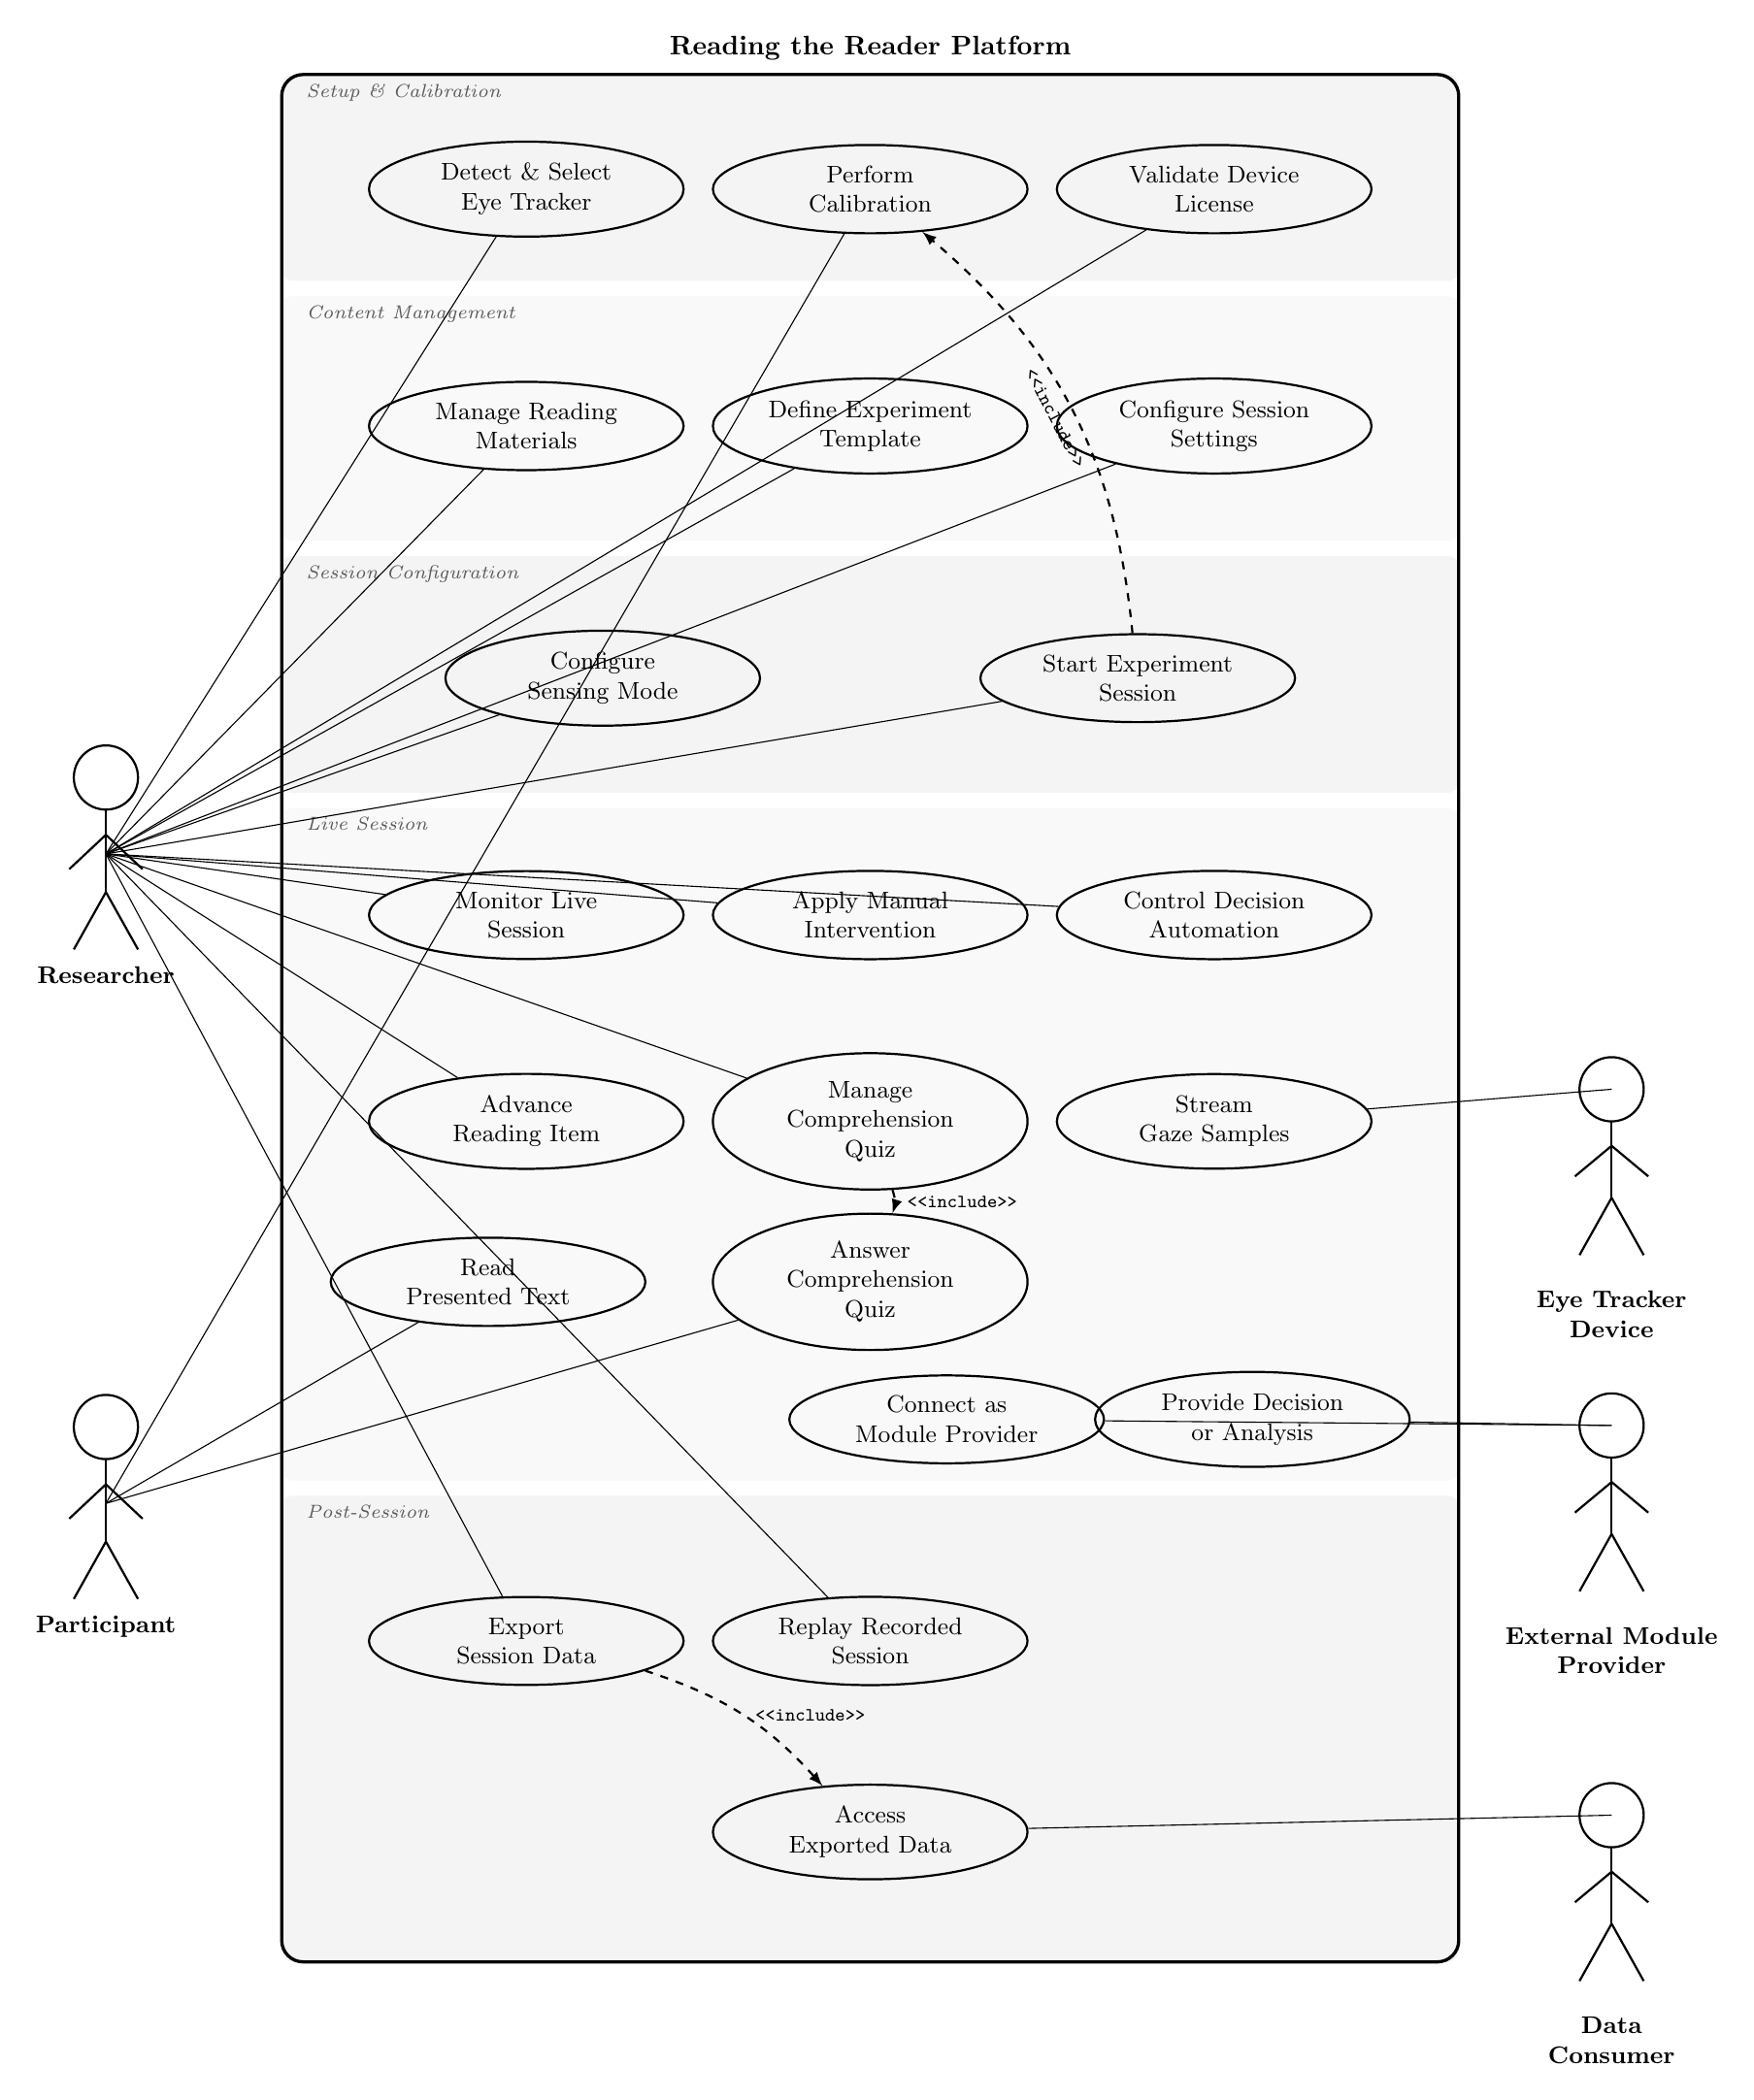
\begin{tikzpicture}[
  %% ── Styles ───────────────────────────────────────────────────────────────
  uc/.style={
    draw, ellipse, thick,
    text width=2.7cm, align=center,
    font=\small, inner sep=3pt,
    minimum height=1.05cm
  },
  inc/.style={
    ->, dashed, >=latex, thick,
    font=\scriptsize
  },
  lbl/.style={
    anchor=north west,
    font=\scriptsize\itshape,
    text=gray!70!black
  },
]

%% ── Group bands (drawn first so they sit behind everything) ──────────────
% Setup & Calibration band
\fill[gray!9, rounded corners=4pt]
  (0.8, 22.5) rectangle (16.2, 25.2);
\node[lbl] at (1.0, 25.2) {Setup \& Calibration};

% Content Management band
\fill[gray!5, rounded corners=4pt]
  (0.8, 19.1) rectangle (16.2, 22.3);
\node[lbl] at (1.0, 22.3) {Content Management};

% Session Configuration band
\fill[gray!9, rounded corners=4pt]
  (0.8, 15.8) rectangle (16.2, 18.9);
\node[lbl] at (1.0, 18.9) {Session Configuration};

% Live Session band — spans researcher controls, system activities,
% participant reading, and provider integration
\fill[gray!5, rounded corners=4pt]
  (0.8, 6.8) rectangle (16.2, 15.6);
\node[lbl] at (1.0, 15.6) {Live Session};

% Post-Session band
\fill[gray!9, rounded corners=4pt]
  (0.8, 0.5) rectangle (16.2, 6.6);
\node[lbl] at (1.0, 6.6) {Post-Session};

%% ── System boundary (drawn on top of bands) ──────────────────────────────
\draw[very thick, rounded corners=8pt]
  (0.8, 0.5) rectangle (16.2, 25.2);
\node[font=\normalsize\bfseries, above=2pt] at (8.5, 25.2)
  {Reading the Reader Platform};

%% ── Use cases ────────────────────────────────────────────────────────────

% Row: Setup & Calibration (y = 23.7)
\node[uc] (uc-detect)    at (4.0,  23.7) {Detect \& Select\\Eye Tracker};
\node[uc] (uc-calibrate) at (8.5,  23.7) {Perform\\Calibration};
\node[uc] (uc-license)   at (13.0, 23.7) {Validate Device\\License};

% Row: Content Management (y = 20.6)
\node[uc] (uc-materials) at (4.0,  20.6) {Manage Reading\\Materials};
\node[uc] (uc-templates) at (8.5,  20.6) {Define Experiment\\Template};
\node[uc] (uc-config)    at (13.0, 20.6) {Configure Session\\Settings};

% Row: Session Configuration (y = 17.3)
\node[uc] (uc-sensing)   at (5.0,  17.3) {Configure\\Sensing Mode};
\node[uc] (uc-start)     at (12.0, 17.3) {Start Experiment\\Session};

% Row: Live Session — researcher-driven controls (y = 14.2)
\node[uc] (uc-monitor)   at (4.0,  14.2) {Monitor Live\\Session};
\node[uc] (uc-intervene) at (8.5,  14.2) {Apply Manual\\Intervention};
\node[uc] (uc-decision)  at (13.0, 14.2) {Control Decision\\Automation};

% Row: Live Session — concurrent runtime activities (y = 11.5)
\node[uc] (uc-advance)   at (4.0,  11.5) {Advance\\Reading Item};
\node[uc] (uc-quiz)      at (8.5,  11.5) {Manage\\Comprehension Quiz};
\node[uc] (uc-stream)    at (13.0, 11.5) {Stream\\Gaze Samples};

% Row: Live Session — participant-side activities (y = 9.4)
\node[uc] (uc-read)      at (3.5,   9.4) {Read\\Presented Text};
\node[uc] (uc-answer)    at (8.5,   9.4) {Answer\\Comprehension Quiz};

% Row: Live Session — external provider activities (y = 7.6)
\node[uc] (uc-connect)   at (9.5,   7.6) {Connect as\\Module Provider};
\node[uc] (uc-provide)   at (13.5,  7.6) {Provide Decision\\or Analysis};

% Row: Post-Session — researcher review and export (y = 4.7)
\node[uc] (uc-export)    at (4.0,   4.7) {Export\\Session Data};
\node[uc] (uc-replay)    at (8.5,   4.7) {Replay Recorded\\Session};

% Row: Post-Session — downstream data access (y = 2.2)
\node[uc] (uc-access)    at (8.5,   2.2) {Access\\Exported Data};

%% ── Actors ───────────────────────────────────────────────────────────────
% Researcher — left side, vertically centred on their fifteen use cases
\def\rX{-1.5} \def\rY{14.0}
\draw[thick] (\rX,     \rY+2.0) circle (0.42);
\draw[thick] (\rX,     \rY+1.58) -- (\rX,  \rY+0.5);
\draw[thick] (\rX,     \rY+0.5)  -- (\rX-0.42, \rY-0.25);
\draw[thick] (\rX,     \rY+0.5)  -- (\rX+0.42, \rY-0.25);
\draw[thick] (\rX,     \rY+1.25) -- (\rX-0.48, \rY+0.80);
\draw[thick] (\rX,     \rY+1.25) -- (\rX+0.48, \rY+0.80);
\node[font=\small\bfseries, align=center, below] at (\rX, \rY-0.35) {Researcher};
\coordinate (researcher) at (\rX, \rY+1.0);

% Participant — left side, lower
\def\pX{-1.5} \def\pY{5.5}
\draw[thick] (\pX,     \pY+2.0) circle (0.42);
\draw[thick] (\pX,     \pY+1.58) -- (\pX,  \pY+0.5);
\draw[thick] (\pX,     \pY+0.5)  -- (\pX-0.42, \pY-0.25);
\draw[thick] (\pX,     \pY+0.5)  -- (\pX+0.42, \pY-0.25);
\draw[thick] (\pX,     \pY+1.25) -- (\pX-0.48, \pY+0.80);
\draw[thick] (\pX,     \pY+1.25) -- (\pX+0.48, \pY+0.80);
\node[font=\small\bfseries, align=center, below] at (\pX, \pY-0.35) {Participant};
\coordinate (participant) at (\pX, \pY+1.0);

% Eye Tracker Device — right side, aligned with gaze-streaming row
\def\eX{18.2} \def\eY{11.5}
\draw[thick] (\eX,     \eY+0.42) circle (0.42);
\draw[thick] (\eX,     \eY)      -- (\eX,  \eY-1.0);
\draw[thick] (\eX,     \eY-1.0)  -- (\eX-0.42, \eY-1.75);
\draw[thick] (\eX,     \eY-1.0)  -- (\eX+0.42, \eY-1.75);
\draw[thick] (\eX,     \eY-0.32) -- (\eX-0.48, \eY-0.72);
\draw[thick] (\eX,     \eY-0.32) -- (\eX+0.48, \eY-0.72);
\node[font=\small\bfseries, align=center, below] at (\eX, \eY-2.1) {Eye Tracker\\Device};
\coordinate (eyetracker) at (\eX, \eY+0.42);

% External Module Provider — right side, aligned with provider activity row
\def\mX{18.2} \def\mY{7.1}
\draw[thick] (\mX,     \mY+0.42) circle (0.42);
\draw[thick] (\mX,     \mY)      -- (\mX,  \mY-1.0);
\draw[thick] (\mX,     \mY-1.0)  -- (\mX-0.42, \mY-1.75);
\draw[thick] (\mX,     \mY-1.0)  -- (\mX+0.42, \mY-1.75);
\draw[thick] (\mX,     \mY-0.32) -- (\mX-0.48, \mY-0.72);
\draw[thick] (\mX,     \mY-0.32) -- (\mX+0.48, \mY-0.72);
\node[font=\small\bfseries, align=center, below] at (\mX, \mY-2.1) {External Module\\Provider};
\coordinate (extprovider) at (\mX, \mY+0.42);

% Data Consumer — right side, bottom
\def\dX{18.2} \def\dY{2.0}
\draw[thick] (\dX,     \dY+0.42) circle (0.42);
\draw[thick] (\dX,     \dY)      -- (\dX,  \dY-1.0);
\draw[thick] (\dX,     \dY-1.0)  -- (\dX-0.42, \dY-1.75);
\draw[thick] (\dX,     \dY-1.0)  -- (\dX+0.42, \dY-1.75);
\draw[thick] (\dX,     \dY-0.32) -- (\dX-0.48, \dY-0.72);
\draw[thick] (\dX,     \dY-0.32) -- (\dX+0.48, \dY-0.72);
\node[font=\small\bfseries, align=center, below] at (\dX, \dY-2.1) {Data\\Consumer};
\coordinate (dataconsumer) at (\dX, \dY+0.42);

%% ── Associations ─────────────────────────────────────────────────────────
% Researcher → fourteen use cases spanning all five bands
% (calibration is performed by the participant, so it is not a researcher association)
\foreach \t in {uc-detect, uc-license,
                uc-materials, uc-templates, uc-config,
                uc-sensing, uc-start,
                uc-monitor, uc-intervene, uc-decision,
                uc-advance, uc-quiz,
                uc-export, uc-replay} {
  \draw (researcher) -- (\t);
}

% Participant → three use cases: calibration fixation, reading, quiz answers
\draw (participant) -- (uc-calibrate);
\draw (participant) -- (uc-read);
\draw (participant) -- (uc-answer);

% Eye Tracker Device → gaze streaming
\draw (eyetracker) -- (uc-stream);

% External Module Provider → provider integration use cases
\draw (extprovider) -- (uc-connect);
\draw (extprovider) -- (uc-provide);

% Data Consumer → exported data access
\draw (dataconsumer) -- (uc-access);

%% ── Include relationships ────────────────────────────────────────────────
% Manage Comprehension Quiz includes Answer Comprehension Quiz
\draw[inc] (uc-quiz)
  to[bend left=18]
  node[right=1pt, font=\scriptsize] {\texttt{<<include>>}}
  (uc-answer);

% Start Experiment Session includes Perform Calibration
\draw[inc] (uc-start)
  to[bend right=22]
  node[below=1pt, font=\scriptsize, sloped] {\texttt{<<include>>}}
  (uc-calibrate);

% Export Session Data includes Access Exported Data
\draw[inc] (uc-export)
  to[bend left=15]
  node[right=1pt, font=\scriptsize] {\texttt{<<include>>}}
  (uc-access);

\end{tikzpicture}%
}
\caption{%
UML use case diagram for the Reading the Reader platform.
Solid lines denote actor--use-case associations;
dashed arrows denote \texttt{<<include>>} dependencies.
Use cases are grouped into five bands:
Setup \& Calibration, Content Management, Session Configuration,
Live Session, and Post-Session.%
}
\label{fig:use-case-diagram}
\end{figure}

\subsection{UC-1: Preparing an Experiment}
\label{sec:uc1}

This scenario traces the \textit{Content Management} and \textit{Setup \&
Calibration} bands of Fig.~\ref{fig:use-case-diagram}, covering all work a
researcher does before a participant arrives.

The preparation begins with the reading library.
Using \textit{Manage Reading Materials}, the researcher creates one or more
materials, each carrying a Markdown content body, descriptive metadata, and an
optional set of comprehension questions.
\textit{Define Experiment Template} then assembles an ordered sequence of those
materials into a reusable session plan; individual items may carry their own
typographic defaults.
Global session parameters (intervention policy, execution mode, and decision
strategy selection) are fixed through \textit{Configure Session Settings}.

Hardware setup follows.
The researcher connects the Tobii eye tracker and uses \textit{Detect \& Select
Eye Tracker} to identify and activate the device.
\textit{Validate Device License} provisions the device licence before any gaze data
is permitted to flow.
\textit{Perform Calibration} runs the calibration point-collection and validation
workflow; the participant fixates on each calibration point in turn while the
system records the correspondence between gaze signal and screen position.
The researcher initiates and oversees this step rather than performing it,
reviewing the resulting quality metrics and repeating the procedure if the
accuracy threshold is not met.
All three hardware steps must pass before the session-start control becomes
available.
This scenario motivates FR2 (Eye-Tracker Detection and Licensing), FR3 (Calibration Integration), FR5 (Reading Content and Presentation), FR14 (Reading Material Library), and FR15 (Experiment Setup Templates).

\subsection{UC-2: Launching and Conducting a Live Reading Session}
\label{sec:uc2}

This scenario spans the \textit{Session Configuration} and \textit{Live Session}
bands and involves three actors: the Researcher, the Participant, and the Eye
Tracker Device.

The researcher selects the active sensing source via \textit{Configure Sensing
Mode}: a physical Tobii device for a real experiment, or mouse-cursor simulation
when running a demonstration without hardware.
\textit{Start Experiment Session} then simultaneously opens the participant
reading interface on a second screen and activates the researcher control panel.
This use case carries a \texttt{<<include>>} dependency on \textit{Perform
Calibration}, enforcing that the calibration gate from UC-1 has been passed.

Once the session is live, the Eye Tracker Device continuously executes
\textit{Stream Gaze Samples}, feeding high-frequency gaze coordinates to the
system in real time.
The Participant executes \textit{Read Presented Text} on their screen while the
researcher uses \textit{Monitor Live Session} to observe the mirrored view,
live gaze highlighting, and a rolling attention summary.

The configured decision strategy processes the incoming gaze and eye-movement
analysis signals.
In automated mode it applies typographic changes directly; in hybrid mode it
emits a proposal that the researcher acts on through \textit{Control Decision
Automation}.
The researcher may also bypass the strategy entirely and apply an immediate change
via \textit{Apply Manual Intervention}.
In all cases the context-preservation mechanism anchors the participant's reading
position so that layout changes do not disorient them.

Where comprehension assessment is required, \textit{Manage Comprehension Quiz}
is activated; this use case carries a \texttt{<<include>>} dependency on
\textit{Answer Comprehension Quiz} on the participant's side, and response
timing is recorded before the session continues.
This scenario motivates FR1 (System Execution and Setup), FR4 (Gaze Data Acquisition and Mapping), FR6 (Researcher Interface), FR7 (Intervention Runtime), FR8 (Decision-Strategy Abstraction), FR9 (Context Preservation), FR11 (Experimental Control), FR13 (Comprehension Quiz), FR16 (Multi-Item Session Sequencing), and FR17 (Sensing Mode Configuration).

\subsection{UC-3: Integrating an External Module Provider}
\label{sec:uc3}

This scenario involves the External Module Provider actor and the two
\textit{Live Session} band use cases on the right side of
Fig.~\ref{fig:use-case-diagram}: \textit{Connect as Module Provider} and
\textit{Provide Decision or Analysis}.

A researcher wishes to evaluate a custom fixation-detection model or an
AI-driven reading-difficulty classifier without modifying the core application.
They launch a compatible external process and connect it to the platform's
dedicated module-provider integration interface.
Upon connection the provider executes \textit{Connect as Module Provider},
declaring its capabilities to the system: whether it processes raw gaze samples
and returns fixation events, or whether it receives decision context and returns
intervention recommendations.

For the remainder of the live session the provider executes \textit{Provide
Decision or Analysis} on an ongoing basis.
Commands it returns pass through the same parameter-validation and
intervention-logging path as built-in strategies, and therefore appear
identically in the session record and in the researcher's control panel.
If the provider disconnects unexpectedly the session is not interrupted: the
platform logs the event and continues with the mode that was active before the
provider connected.
This scenario demonstrates that the extensibility requirement is fulfilled at
the protocol level: new decision and analysis algorithms are delivered as
separate processes communicating over a documented interface, and the core
codebase is left unmodified.
This scenario motivates FR18 (Eye-Movement Analysis Layer) and FR19 (External Module Provider Framework).

\subsection{UC-4: Reviewing and Exporting Session Data}
\label{sec:uc4}

This scenario covers the remaining \textit{Post-Session} use cases and involves
both the Researcher and the Data Consumer actor.

When a session ends the researcher uses \textit{Export Session Data} to produce
a structured session record.
This use case carries a \texttt{<<include>>} dependency on \textit{Access Exported
Data}: the export operation both writes the artefact to the server and immediately
makes it available for retrieval.
The record bundles raw gaze samples, derived fixation and saccade events, all
intervention events with source attribution and timestamps, comprehension quiz
results, calibration metadata, and the complete typographic configuration,
in a structured machine-readable format.

The researcher may then load any saved export into the platform via
\textit{Replay Recorded Session}, which reconstructs the reading interface with
animated gaze-path playback, intervention markers on the timeline, and
variable-speed playback controls.
Previously saved exports are listed in the application and are reloadable without
manual file management, satisfying the need to review multiple sessions across a
study.

Independently of the researcher, a Data Consumer executes \textit{Access Exported
Data} to retrieve the record for offline analysis.
Because the export alone is sufficient to reconstruct the full sequence of
sensing, analysis, and intervention events, this use case is the primary
mechanism through which the reproducibility requirement is satisfied.
This scenario motivates FR10 (Real-Time Performance Monitoring), FR12 (Logging and Export), FR21 (Session Replay Playback), and FR22 (Session State Recovery).

\subsection{End-to-End Session Workflow}
\label{sec:activity-session}

While the use case diagram in Fig.~\ref{fig:use-case-diagram} captures actor associations, it does not express the order in which activities occur, the conditions under which the workflow branches, or the activities that proceed concurrently during a live session.
Fig.~\ref{fig:activity-session} traces the control flow of a complete experimental session, synthesising the preparation path of UC-1 and the live path of UC-2 into a single workflow, partitioned into swimlanes that show which actor performs each activity.
The diagram remains at the analysis level: every node denotes an activity, every branch a condition, and every lane an actor, with no reference to system components or internal mechanisms.

\begin{figure}[p]
\centering
\resizebox{!}{0.86\textheight}{%
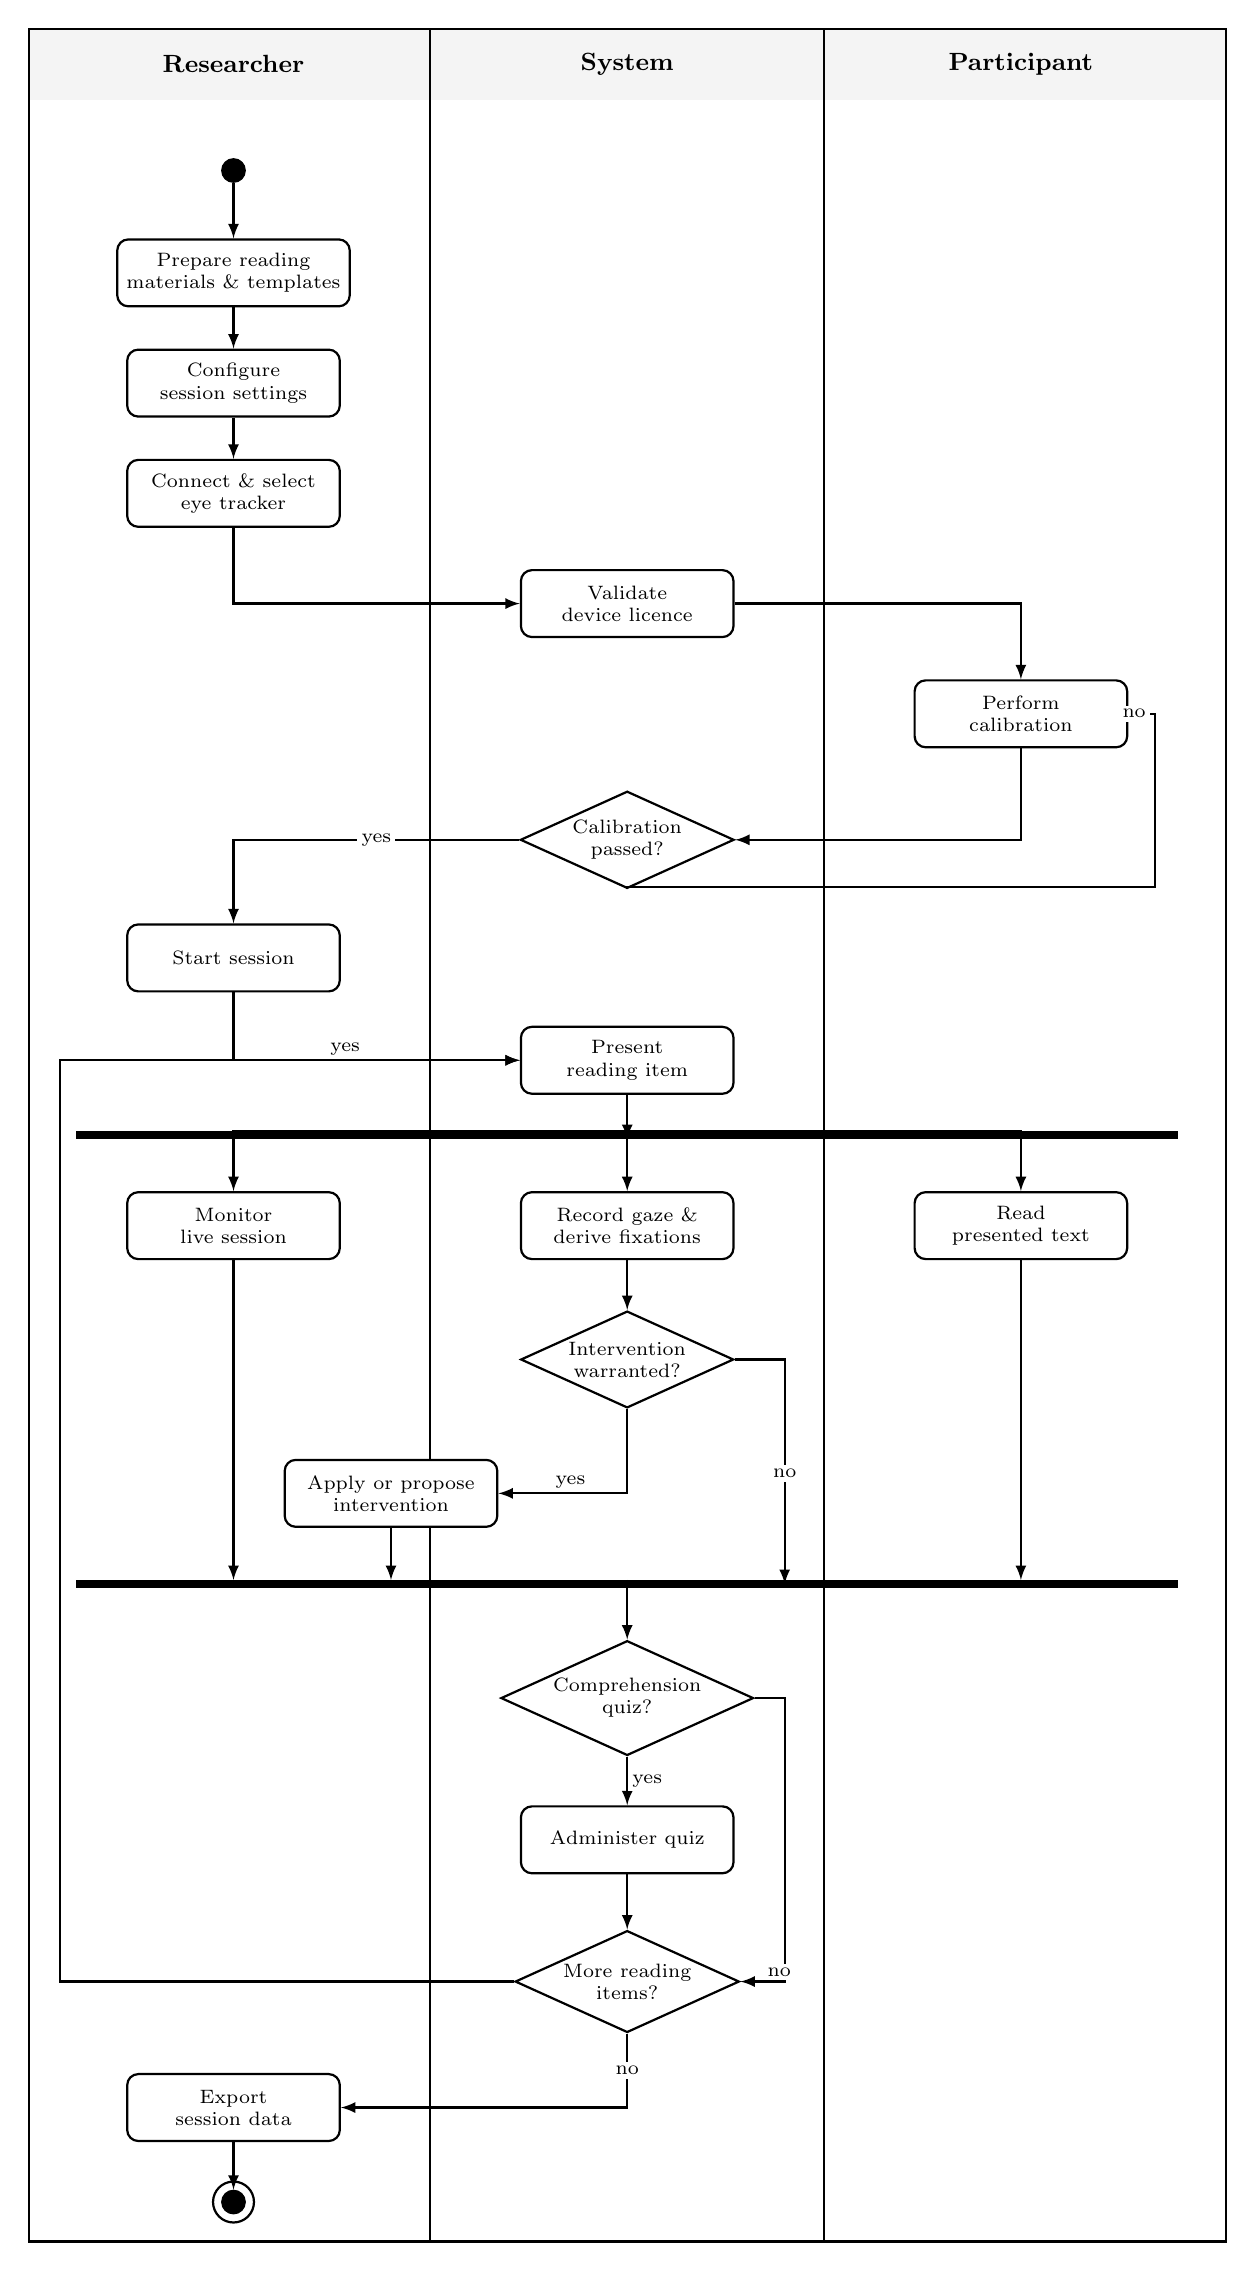
\begin{tikzpicture}[
  act/.style={draw, rounded corners=4pt, thick, minimum width=2.7cm,
              minimum height=0.85cm, align=center, font=\scriptsize, fill=white},
  dec/.style={draw, diamond, aspect=2.2, thick, inner sep=1pt, align=center,
              font=\scriptsize, fill=white},
  term/.style={draw, circle, fill=black, minimum size=0.3cm, inner sep=0},
  flow/.style={->, >=latex, thick},
  elbl/.style={font=\scriptsize, fill=white, inner sep=1.5pt},
  lane/.style={font=\small\bfseries}
]

%% ── Lane backdrop, dividers, headers ───────────────────────────────────────────
\fill[gray!9] (-2.6, 1.0) rectangle (12.6, 1.9);
\draw[thick] (-2.6,1.9) rectangle (12.6,-26.2);
\draw[thick] (2.5, 1.9) -- (2.5,-26.2);
\draw[thick] (7.5, 1.9) -- (7.5,-26.2);
\node[lane] at (0,1.45)  {Researcher};
\node[lane] at (5,1.45)  {System};
\node[lane] at (10,1.45) {Participant};

%% ── Nodes (placed in the lane of the actor that performs them) ──────────────────
\node[term] (start)    at (0,  0.1)  {};
\node[act]  (prepare)  at (0, -1.2)  {Prepare reading\\materials \& templates};
\node[act]  (config)   at (0, -2.6)  {Configure\\session settings};
\node[act]  (connect)  at (0, -4.0)  {Connect \& select\\eye tracker};
\node[act]  (validate) at (5, -5.4)  {Validate\\device licence};
\node[act]  (calib)    at (10,-6.8)  {Perform\\calibration};
\node[dec]  (d1)       at (5, -8.4)  {Calibration\\passed?};
\node[act]  (startses) at (0, -9.9)  {Start session};
\node[act]  (present)  at (5, -11.2) {Present\\reading item};

% Fork bar (spans the live phase)
\fill (-2.0,-12.2) rectangle (12.0,-12.1);

\node[act]  (monitor)  at (0, -13.3) {Monitor\\live session};
\node[act]  (record)   at (5, -13.3) {Record gaze \&\\derive fixations};
\node[act]  (read)     at (10,-13.3) {Read\\presented text};

\node[dec]  (d2)       at (5, -15.0) {Intervention\\warranted?};
\node[act]  (apply)    at (2.0,-16.7) {Apply or propose\\intervention};

% Join bar
\fill (-2.0,-17.9) rectangle (12.0,-17.8);

\node[dec]  (d3)       at (5, -19.3) {Comprehension\\quiz?};
\node[act]  (quiz)     at (5, -21.1) {Administer quiz};
\node[dec]  (d4)       at (5, -22.9) {More reading\\items?};
\node[act]  (export)   at (0, -24.5) {Export\\session data};
\node[term] (end0)     at (0, -25.7) {};
\draw[thick] (end0) circle (0.26);

%% ── Sequential flow ───────────────────────────────────────────────────────────
\draw[flow] (start)    -- (prepare);
\draw[flow] (prepare)  -- (config);
\draw[flow] (config)   -- (connect);
\draw[flow] (connect.south) |- (validate.west);
\draw[flow] (validate.east) -| (calib.north);
\draw[flow] (calib.south) |- (d1.east);
\draw[flow] (d1.west) -| (startses.north) node[elbl,pos=0.25]{yes};
\draw[flow] (startses.south) |- (present.west);

% Calibration retry (no): up the right margin back to the participant
\draw[flow] (d1.south) -- (5,-9.0) -- (11.7,-9.0) -- (11.7,-6.8) -- (calib.east)
  node[elbl, pos=0.78]{no};

% Fork out into the three concurrent lanes
\draw[flow] (present) -- (5,-12.2);
\draw[flow] (5,-12.1) -| (monitor.north);
\draw[flow] (5,-12.1) -- (record.north);
\draw[flow] (5,-12.1) -| (read.north);

% Middle lane: record -> intervention -> join
\draw[flow] (record) -- (d2);
\draw[flow] (d2.south) |- (apply.east) node[elbl,above,pos=0.72]{yes};
\draw[flow] (d2.east) -- (7.0,-15.0) -- (7.0,-17.85) node[elbl,above,pos=0.55]{no};
\draw[flow] (apply.south) -- (2.0,-17.8);

% Side lanes into the join
\draw[flow] (monitor.south) -- (0,-17.8);
\draw[flow] (read.south) -- (10,-17.8);

% After join
\draw[flow] (5,-17.8) -- (d3);
\draw[flow] (d3.south) -- (quiz) node[elbl,right,pos=0.5]{yes};
\draw[flow] (quiz.south) -- (d4);
\draw[flow] (d3.east) -- (7.0,-19.3) -- (7.0,-22.9) -- (d4.east) node[elbl,above,pos=0.12]{no};
\draw[flow] (d4.south) |- (export.east) node[elbl,pos=0.25]{no};
\draw[flow] (export) -- (end0);

% Multi-item loop (yes): up the left margin to the next reading item
\draw[flow] (d4.west) -- (-2.2,-22.9) -- (-2.2,-11.2) -- (present.west)
  node[elbl,above,pos=0.62]{yes};

\end{tikzpicture}%
}
\caption{%
Swimlane activity diagram for a complete experimental session, partitioned by
actor into Researcher, System, and Participant lanes.
Rounded boxes are activities and diamonds are decisions; the solid horizontal
bars denote the fork and join that bound the concurrent activities of the live
reading phase.
Each activity sits in the lane of the actor that performs it: the researcher
prepares and operates the session, the participant performs the calibration and
reads, and the system validates, senses, and adapts.
The intervention activity straddles the researcher and system lanes because an
intervention may be applied automatically by the system or proposed by the system
and approved by the researcher.
The diagram stays at the analysis level, describing what happens, under what
conditions, and by whom, rather than how the system is structured internally.%
}
\label{fig:activity-session}
\end{figure}

Two readiness gates structure the flow.
Calibration repeats until its quality threshold is met, and a reading item cannot begin until calibration has passed and the device is licensed.
During each reading item, three activities proceed concurrently: the participant reads the presented text, the system records gaze and derives fixation events, and the researcher monitors the live session.
Within the sensing activity an intervention is applied or proposed only when the current reading state warrants it, reflecting the configurable execution modes captured in FR11.
The outer loop returns to the next reading item until the experiment template is exhausted, after which the session data is exported for later analysis.

% ---------------------------------------------------------------

